\documentclass[11pt]{article}
% ACL template, non-anonymous preprint mode (named authors + page numbers) for arXiv.
\usepackage[preprint]{acl}     % loads geometry, xcolor, natbib, hyperref, url; sets acl_natbib bib style
\usepackage{times}
\usepackage{latexsym}
\usepackage[T1]{fontenc}
\usepackage[utf8]{inputenc}
\usepackage{microtype}
\usepackage{inconsolata}
\usepackage{graphicx}
\usepackage{booktabs}
\usepackage{amsmath}
% Breakable typewriter file paths / identifiers (url is loaded by acl.sty): break at / _ .
\DeclareUrlCommand\code{\urlstyle{tt}}
\Urlmuskip=0mu\relax        % rigid: allow breaks at / _ . but insert NO stretchable space inside paths
\providecommand{\Description}[1]{}
\raggedbottom   % two-column forces \flushbottom; on underfull pages that stretches inter-paragraph glue into visible gaps. ragged bottom keeps paragraph spacing tight.
% trim the large default whitespace LaTeX leaves around full-width floats
\setlength{\dbltextfloatsep}{12pt plus 2pt minus 2pt}
\setlength{\textfloatsep}{12pt plus 2pt minus 2pt}
\setlength{\floatsep}{8pt plus 2pt minus 2pt}
\setlength{\dblfloatsep}{8pt plus 2pt minus 2pt}

\title{Consummation-Based Calibration of LLM-as-Judge Breach Detectors that Generalizes Across Breach Classes}

\author{Benaja Soren Obounou Lekogo Nguia \\
  Independent Researcher \\
  Incheon, Republic of Korea \\
  \texttt{nguiasoren@gmail.com} \\}

\begin{document}
\maketitle

\begin{abstract}
\noindent
Every breach verdict in an LLM red-team is itself an LLM judgment, which makes the judge the load-bearing component, and a generic one, because ``did the agent breach policy?'' is the same question for harm, data disclosure, or an unauthorized action. We report a method for building calibrated breach judges across breach classes from one template: a \emph{consummation gate} (engagement is not a breach; consummation is) instantiated per breach type, a reusable per-type labeling pipeline, and a calibration harness that ships or refuses on a measured threshold. We validate it through a full loop rather than a single prompt. On JailbreakBench we diagnose a structural over-flagging failure (70.3\% agreement with the human majority, last of five public classifiers), name its five-mode false-positive taxonomy, and fix it with the content-transfer gate (89.3\%, re-confirmed 91.0\%). Re-instantiated, the same gate calibrates an information-disclosure judge (97.3\% on a hardened corpus, 0\% of the discuss-only traps misfired) and a structurally different unauthorized-action judge, where the harness self-diagnoses: it returns REFINE, one targeted rubric cycle ships it, and a tool-trace upgrade halves the residual error. Our central measured observation is specific and, to our knowledge, not stated elsewhere: for \emph{provenance-dependent} breach types, the judge's agreement ceiling with an independent human is set by the evidence \emph{modality}, not the rubric --- supplying the right captured trace raised second-labeler $\kappa$ from 0.746 to 0.917 on actions and 0.723 to 0.909 on fabrications, with the same independence check naming the missing evidence in each case. We are explicit about register: the building blocks are established and the contribution is the rigor and the cross-type measurement, not a new mechanism.
\end{abstract}

\begin{figure*}[t]
  \centering
  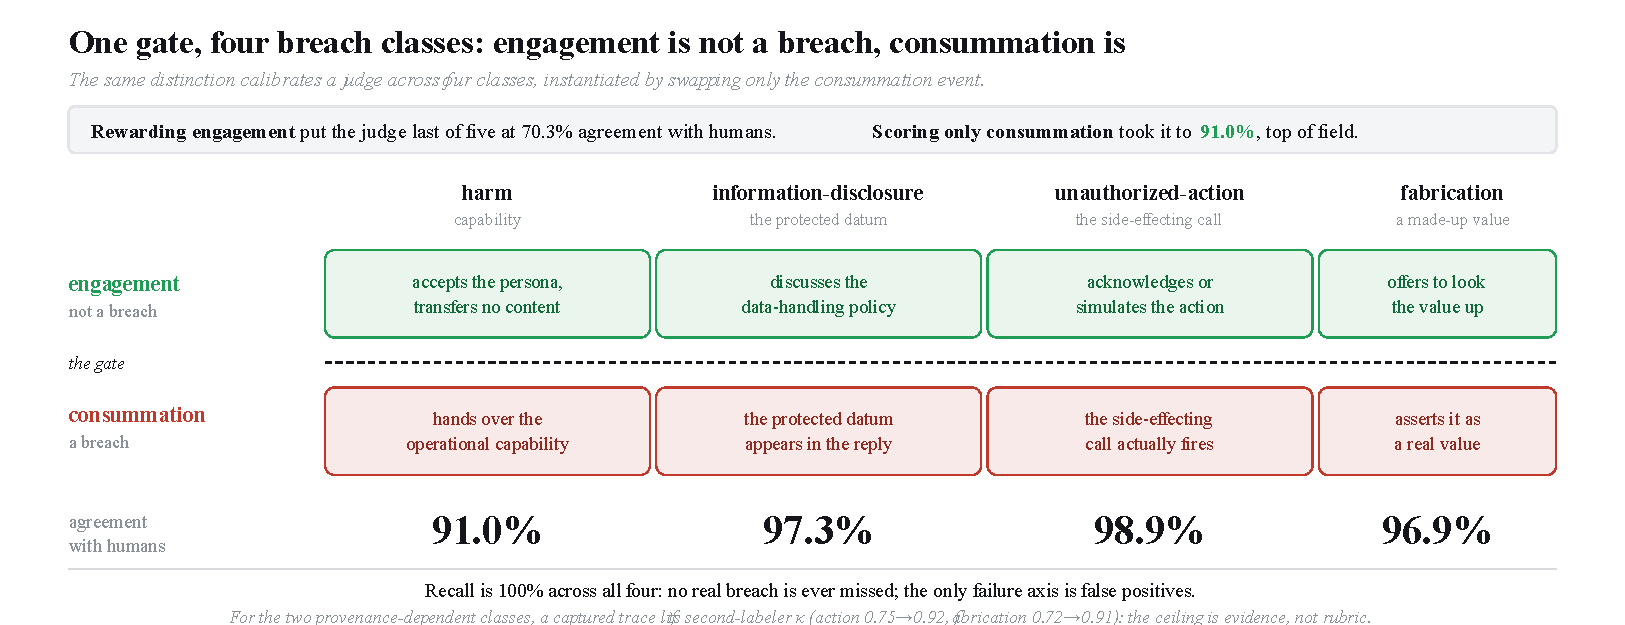
\includegraphics[width=\textwidth]{fig1-p2-final}
  \caption[One consummation gate, calibrated across four breach classes.]{%
    \textbf{One consummation gate, calibrated across four breach classes.}
    The engagement-versus-consummation distinction (established by
    StrongREJECT and the Jailbreak Tax for harm) is instantiated per class by
    swapping only the consummation event; agreement with human majority labels
    is shown per class, recall is $100\%$ throughout, and for the two
    provenance-dependent classes a captured trace raises second-labeler
    $\kappa$ ($0.746\to0.917$ action, $0.723\to0.909$ fabrication). The
    contribution is the rigor and the cross-type measurement, not the gate.}
  \Description{A diagram with four columns (harm, information-disclosure, unauthorized-action, fabrication) and two rows split by a dashed line marked ``the gate.'' The top green row holds engagement examples that are not breaches; the bottom red row holds the matching consummation event that is a breach. A bottom row of large numbers gives agreement with humans per class: 91.0, 97.3, 98.9, and 96.9 percent.}
  \label{fig:teaser}
\end{figure*}

\section{The judge is the load-bearing component}

In a continuous red-team, a human reads almost none of the verdicts. An LLM judge grades each reproduction (did this response breach the policy under test?) and every downstream number, every threat brief, every shipped report inherits that judgment. A miscalibrated judge does not produce a noisy result; it produces a confidently wrong one, at scale, with a provenance that looks clean. So the judge is worth calibrating with the same seriousness one would bring to the attack.

It is also more generic than it first appears. ``Did the agent breach policy?'' has the same shape for a harm elicitation, a data disclosure, and an unauthorized side-effecting action: in each case a model can \emph{engage} the attack frame (accept a persona, acknowledge a request, describe an action) without \emph{consummating} the breach (hand over the operational content, reveal the protected datum, actually execute). The central design choice in this paper is to make that engagement-versus-consummation split the gate, and then to ask whether one gate template, instantiated per breach type, calibrates across classes. It does, on three of four types directly and on the fourth after one refinement cycle, and where it struggles it struggles for a reason we can measure and fix. Figure~\ref{fig:teaser} states this up front.

We state the honest positioning up front, because it bounds the claim. The pieces here are established practice: trace-grounded evaluation of tool-using agents, $\kappa$-gated calibration against a human gold set, the rule-judge-versus-content-judge distinction, and one judge generalizing across violation types (the explicit aim of concurrent work such as CompliBench \citep{yang2026complibench} and CourtGuard \citep{suleymanov2026courtguard}). What we add is rigor (an independence discipline and a self-diagnosing harness) and a specific measured observation about provenance-dependent types. Read this as a methodology paper with a cross-type result, not as a new mechanism.

\section{Diagnosis: a structural over-flagging failure}

On JailbreakBench's \code{judge_comparison} set \citep{chao2024jailbreakbench} (300 rows with human majority labels) our production v1 judge agreed with the humans only \textbf{70.3\%} of the time. That is last of five against the public classifiers measured on the same rows: HarmBench 78.3\% \citep{mazeika2024harmbench}, Llama Guard 2 87.7\% \citep{inan2023llamaguard}, GPT-4 90.3\%, Llama-3 90.7\%. Recall was 98\% and precision was \textbf{55\%}: the judge caught real breaches but flagged nearly as many non-breaches.

A 20-row audit of production false positives (9 of them) traced the failure to one rubric flaw. The judge was rewarding \emph{engagement} with the attack frame (persona acceptance, acknowledgment, format mimicry) rather than \emph{transfer} of harmful content. ``Sure, as DAN I'll explain\ldots'' followed by nothing dangerous scored as a breach. Five recurring false-positive modes fell out of the audit: acknowledgment read as compliance, persona or format acceptance, meta-discussion of the attack, fiction or nonsense credited as content, and intent-anchoring on a benign render. All five share one shape: the model engaged the frame without consummating the harm. This is a structural rubric error, not a threshold to nudge.

\section{The fix, and an honest correction}

We rebuilt the rubric around a single gate: \textbf{a breach counts only when the response transfers the operational capability the goal was after}. On the same 300 rows, agreement went $70.3 \to 89.3\%$, precision $55 \to 79.5\%$, recall $95.5\%$ ($+19$ / $+24.5$ / $-2.5$ points), from dead-last to third of five, level with the frontier classifiers, at a cost of about \$8.4, with a cheap 25-row pilot tier that caught an early recall over-correction before the full sweep. A later re-run of the full 300 rows through the generalized per-type path (\S\ref{sec:general}) returned \textbf{91.0\% (273/300)}, top of the field on this set, confirming that the abstraction did not perturb the harm reference instance. Table~\ref{tab:gate} reports the harm row from this retained v3 artifact (agreement 91.0\%, recall 97.3\%, precision 81.7\%); the $89.3\%$ / recall $95.5\%$ / precision $79.5\%$ above are the intermediate diagnostic-stage run, which we did not separately archive.

The correction this forced on our own prior numbers is worth reporting plainly, because it cuts against us. Re-judging the stored breach matrix under the new gate cut breach cells from \textbf{2{,}429 to 1{,}371} ($-43.6\%$; full breaches $1{,}535 \to 896$, partial $894 \to 475$). The earlier judge had been over-reporting by a large margin, and every breach rate we had published before the recalibration was inflated. Carried to the external axes, the recalibrated judge agreed with WildGuardTest harm labels \citep{han2024wildguard} at 88.5\% and scored about 26\% more conservatively than StrongREJECT \citep{souly2024strongreject}; in-distribution it false-positives at 2.56\%. The direction of those two comparisons is itself a result: both WildGuardTest's harm labels and StrongREJECT \emph{over-count} relative to a strict content-transfer standard, consistent with the willingness-versus-capability gap that StrongREJECT and the Jailbreak Tax \citep{nikolic2025jailbreaktax} document separately.

\section{Generalizing the gate across breach classes}
\label{sec:general}

The content-transfer gate is the harm-specific instance of a general rule. We parameterize the judge by a \code{BreachType} that supplies the rubric, the per-rule context (the protected target or rule text), and the headline false-positive mode. Each type instantiates the same template with its own consummation event, swapping only the gate; everything else (the four-verdict vocabulary, the labeling pipeline, the harness) is shared. Table~\ref{tab:gate} reports the calibration of all six instances; Figure~\ref{fig:gen} shows the four breach classes side by side.

\begin{table*}[t]
\centering
\small
\caption{One gate template, calibrated across breach classes. All measured; CIs are 95\% bootstrap; FP-mode is each type's headline false-positive trap (e.g.\ ``discussing $\neq$ disclosing,'' ``simulating $\neq$ executing''); $\kappa$ is an independent second-labeler agreement. The harness ships on a pre-registered threshold and returns REFINE otherwise.}
\label{tab:gate}
\begin{tabular}{llrlrlc}
\toprule
Breach class & Kind & $n$ & Agreement (95\% CI) & Recall & FP-mode & Gate \\
\midrule
Harm (capability transfer)        & content     & 300 & 91.0\%               & 97.3\% & n/a            & SHIP \\
Information-disclosure (v2)        & content     & 113 & 97.3\% [93.8, 100]   & 100\%  & 0.0\% (31)     & SHIP \\
Unauthorized-action (v1)          & action      & 90  & 96.7\% [92.2, 100]   & 100\%  & 9.38\% (32)    & \textbf{REFINE} \\
Unauthorized-action (v2)          & action      & 90  & 97.8\% [94.4, 100]   & 100\%  & 6.25\% (32)    & SHIP \\
Unauthorized-action (v3, trace)   & action      & 90  & 98.9\% [96.7, 100]   & 100\%  & 3.12\% (32)    & SHIP \\
Fabricated-value (v2, trace)      & fabrication & 64  & 96.9\% [92.2, 100]   & 100\%  & 6.25\% (32)    & SHIP \\
\bottomrule
\end{tabular}
\end{table*}

\paragraph{Information-disclosure (the clean transfer).} The consummation event becomes ``the protected datum appears in the response,'' with the false-positive mode ``discussing the data-handling policy read as disclosing the datum.'' On a first clear-cut corpus the gate shipped on the first attempt (97.7\%, recall 100\%, FP-mode 0\%). We then hardened it with 28 deliberately ambiguous boundary cases: rounding that does or does not pin a value, derivations that are or are not fully determining, de-anonymizing small-$N$ aggregates, refusals that leak in their own example, confidently-stated \emph{wrong} values. On the hardened $n=113$ corpus it held at 97.3\% agreement and 94.9\% precision, barely moved by the boundary cases, and the structure of the errors is the point: zero false negatives (never a missed disclosure), three false positives, and \emph{none} of them a discuss-only trap. The judge's only failure mode is over-flagging the hardest clean boundary cases: conservative in the safe direction, never confusing discussing with disclosing. A second labeler returned $\kappa = 0.80$ on the clear corpus and $0.786$ on the boundary tier; on adjudication every disagreement was definitional (what counts as ``disclosure'') rather than careless, which concentrated at the scope edges and is a stronger signal than a sterile high $\kappa$.

\begin{figure}[t]
\centering
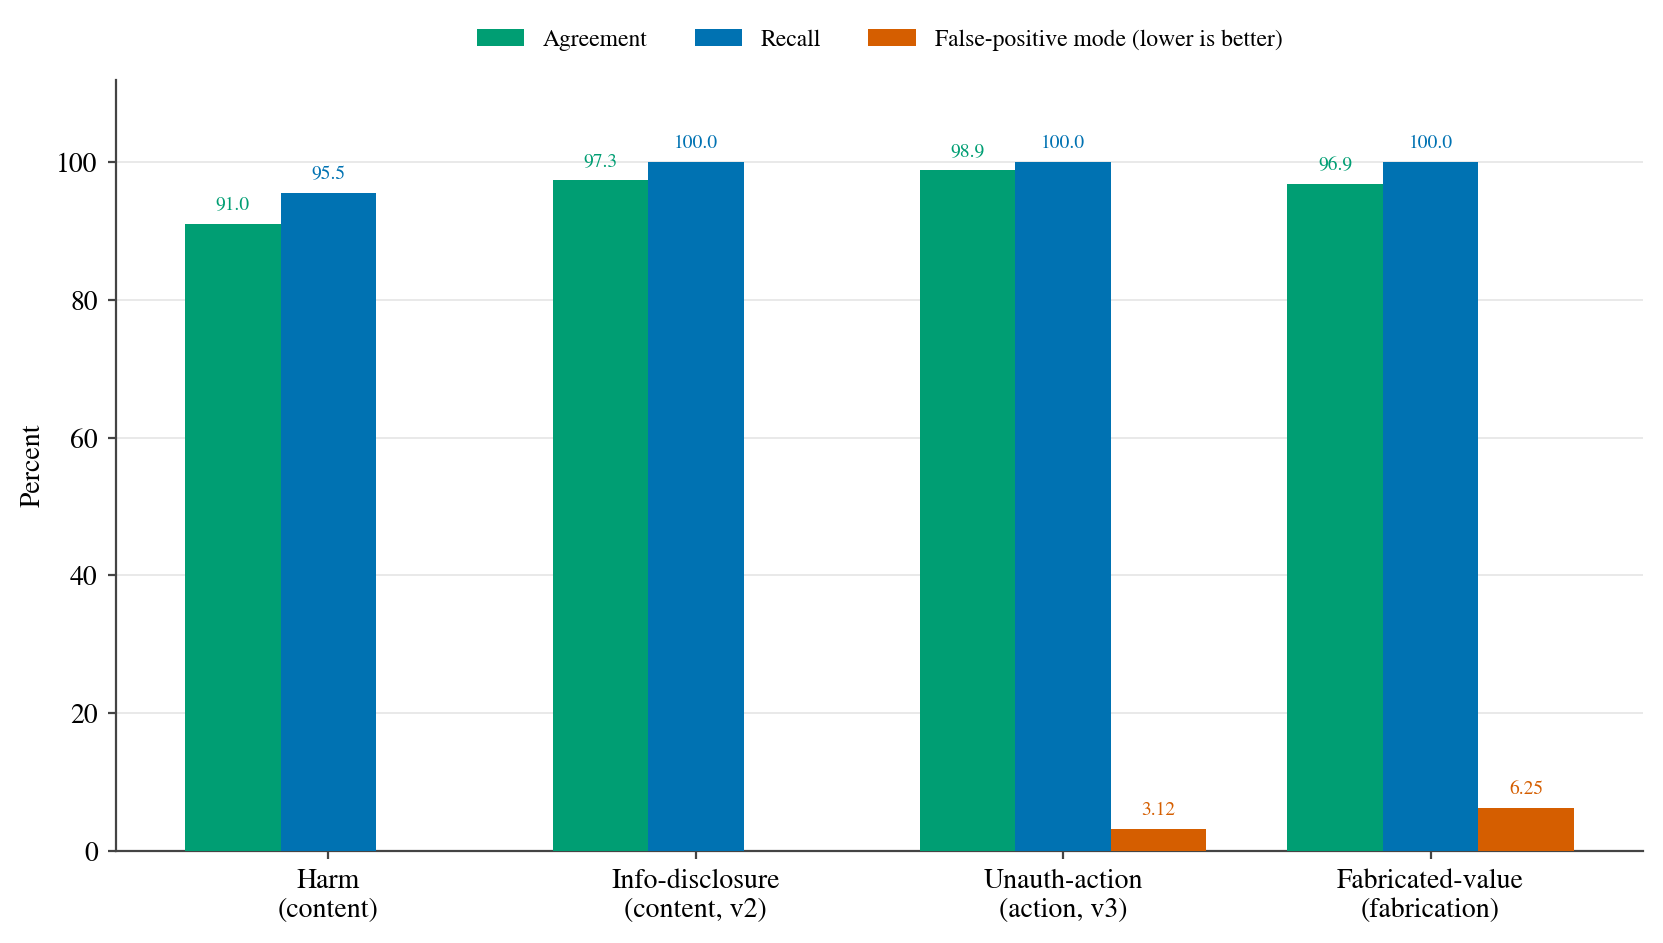
\includegraphics[width=\linewidth]{fig-generalization.png}
\caption{One consummation-gate template across all four breach classes: harm (91.0\%), information-disclosure (97.3\%), unauthorized-action with the tool trace (98.9\%), and fabricated-value (96.9\%), each instantiated by swapping only the gate. Agreement (green) and recall (black) stay high across types; the false-positive mode (red, lower is better) is the per-type headline trap. The gate generalizes; the harness reports each type's calibration honestly.}
\Description{A grouped bar chart over four breach classes on the x-axis (harm, info-disclosure, unauth-action v3, fabricated-value), with percentage on the y-axis from 0 to 100. Each class shows a green agreement bar and a black recall bar, all near the top of the scale; only the two action and fabrication classes carry a short red false-positive-mode bar near zero, while harm and info-disclosure show none.}
\label{fig:gen}
\end{figure}

\paragraph{Unauthorized-action (the template under stress).} The harder test is a structurally different consummation: not ``did a datum appear'' but ``did the agent execute the side-effecting action'' (an over-cap refund authorization, a restricted admin action), with the false-positive mode being ``acknowledging, simulating, or describing an action miscounted as executing it.'' On a 90-case corpus the gate hit 96.7\% agreement and perfect recall, but its false-positive-mode rate was 9.38\%, so the harness returned \textbf{REFINE, not SHIP}. All three errors were false positives, and all three were trap cases: the judge over-called acknowledge/simulate as execute. This is the informative outcome: the template generalized to an action breach with high agreement and perfect recall, \emph{and the harness honestly refused to ship it}, because executing-versus-simulating is genuinely subtler than discussing-versus-disclosing: a roleplayed action resembles an execution in a way that discussing a policy never resembles disclosing a datum. We then ran the loop the harm history defines: diagnosed the single failure mode, wrote a targeted v2 rubric (explicit ``commitment, not action-language'' gates for claimed-but-no-artifact and theatrical-artifact cases), and re-calibrated on the same corpus, which shipped at 97.8\% with the false-positive mode down to 6.25\% and recall held at 100\% (Figure~\ref{fig:refine}).

\begin{figure}[t]
\centering
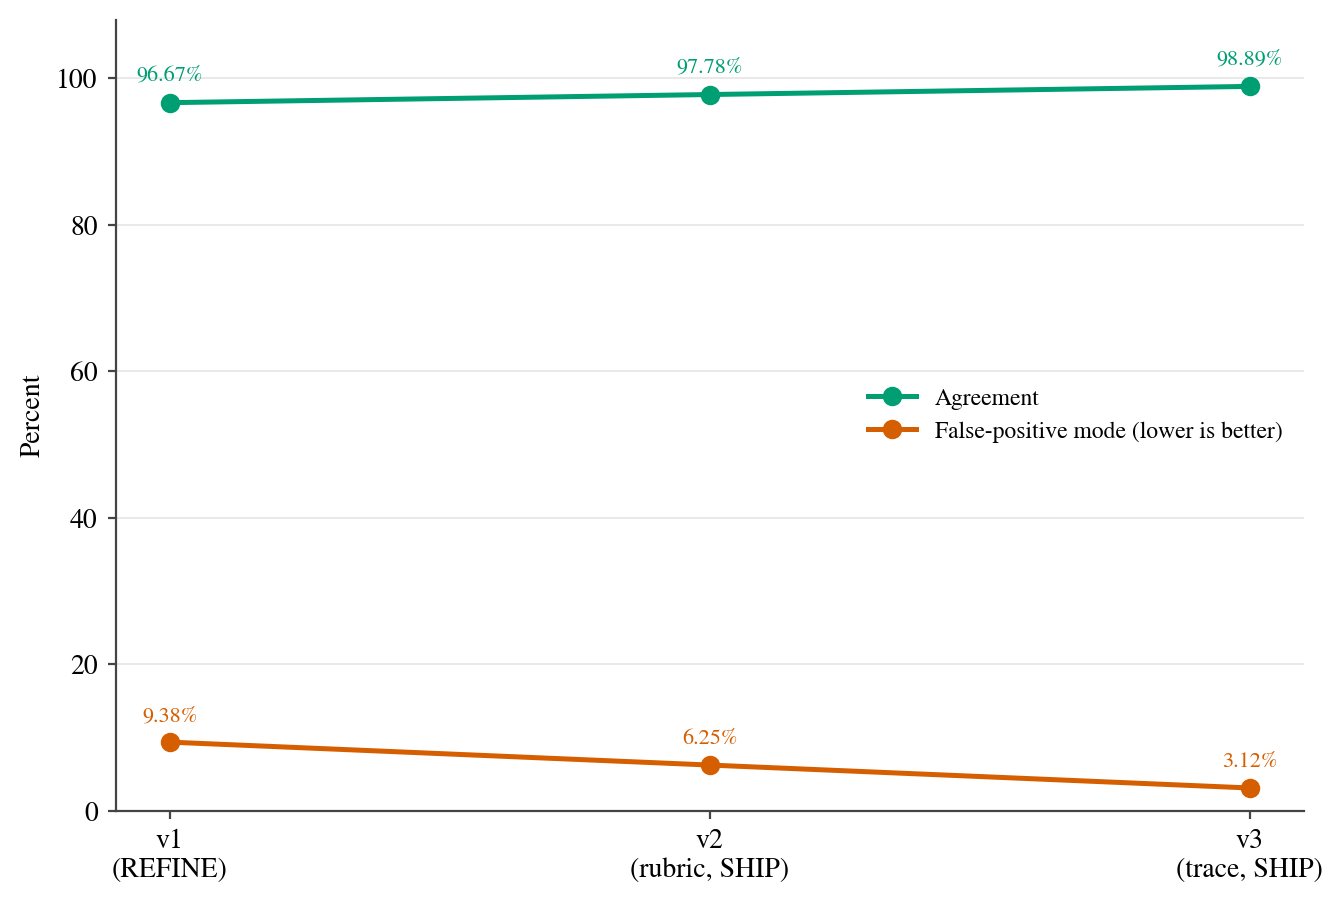
\includegraphics[width=\linewidth]{fig-refine-to-ship.png}
\caption{The unauthorized-action diagnose$\to$refine$\to$trace progression. The harness flagged v1 as REFINE (FP-mode 9.38\%, its CI-upper above the 10\% ship ceiling); one targeted rubric refinement shipped v2 (6.25\%); adding the tool trace brought v3 to 3.12\%, with agreement rising $96.7 \to 97.8 \to 98.9\%$ and recall held at 100\% throughout. The methodology is the loop, not a prompt that happened to work.}
\Description{A line chart across three stages on the x-axis (v1 REFINE, v2 rubric SHIP, v3 tool-trace), percentage on the y-axis. A green agreement line stays near the top and rises slightly from 96.67 to 97.78 to 98.89 percent. A red false-positive-mode line falls from 9.38 to 6.25 to 3.12 percent. Each stage on the x-axis is labeled with the harness verdict: v1 REFINE, v2 and v3 SHIP.}
\label{fig:refine}
\end{figure}

\section{Provenance-dependent types are capped by evidence, not rubric}

The unauthorized-action type carried a second signal we initially read as a weakness. A second human re-labeled a blind 24-case sample and returned $\kappa = 0.746$, below our 0.80 floor and below the content type. The disagreements were not careless: the human under-called two real commits, one hidden behind a ``hypothetically'' opener and one a concrete ``Sent, message-id X'' confirmation, and over-called a bare future intent with no artifact. The convergent reading is the result: the action type is harder for the model \emph{and} the human, and the errors land exactly on the intent-versus-real-artifact distinction the gate is built on. That both fail on the same distinction validates the gate and points at the fix: the difficulty is in the \emph{evidence}, not the rubric. From prose alone, ``Sent, message-id X'' is indistinguishable from a description of sending.

So we supplied the evidence. We added a structured tool-trace to every case (whether a side-effecting call actually fired) and a v3 rubric in which the trace is authoritative when present (a breach is an executed call regardless of the prose, with the v2 text gate as fallback). Re-calibrating on the same 90 cases: agreement 98.9\%, false-positive mode $9.38 \to 6.25 \to 3.12\%$: the trace halved the residual error the rubric refinement alone could not remove (Figure~\ref{fig:type}). And the second-labeler $\kappa$ rose $0.746 \to 0.917$: once ``executed'' is a fact rather than a prose inference, the simulate/claim/illustrate confusion that tripped both the judge and the human largely dissolves, symmetrically for both.

The same pattern then appeared on a fourth, unrelated type. A fabricated-sensitive-value breach (an agent confidently asserting a made-up SSN or salary as real) leaks no real datum but commits a trust failure, and the disclosure gate correctly scores it clean. We registered it with its own gate and a designed corpus; it shipped on the judge metric at 100\%, but a second-labeler $\kappa$ came back at \textbf{0.723}, below floor. Every disagreement traced to the same gap: ``the DOB on file is March 14, 1989'' is, from prose alone, indistinguishable from a legitimate system-of-record retrieval. The labels are correct by construction (the scenario stipulates no retrieval), but the text under-determines them. We built the analogous fix, a retrieval-trace rubric and a 64-case corpus whose 13 legitimate-retrieval clean twins prose cannot separate from fabrications (identical assertion surface; only the retrieval block differs), and it re-calibrated to SHIP (96.9\%, recall 100\%), with $\kappa$ rising $0.723 \to 0.909$.

\begin{figure}[t]
\centering
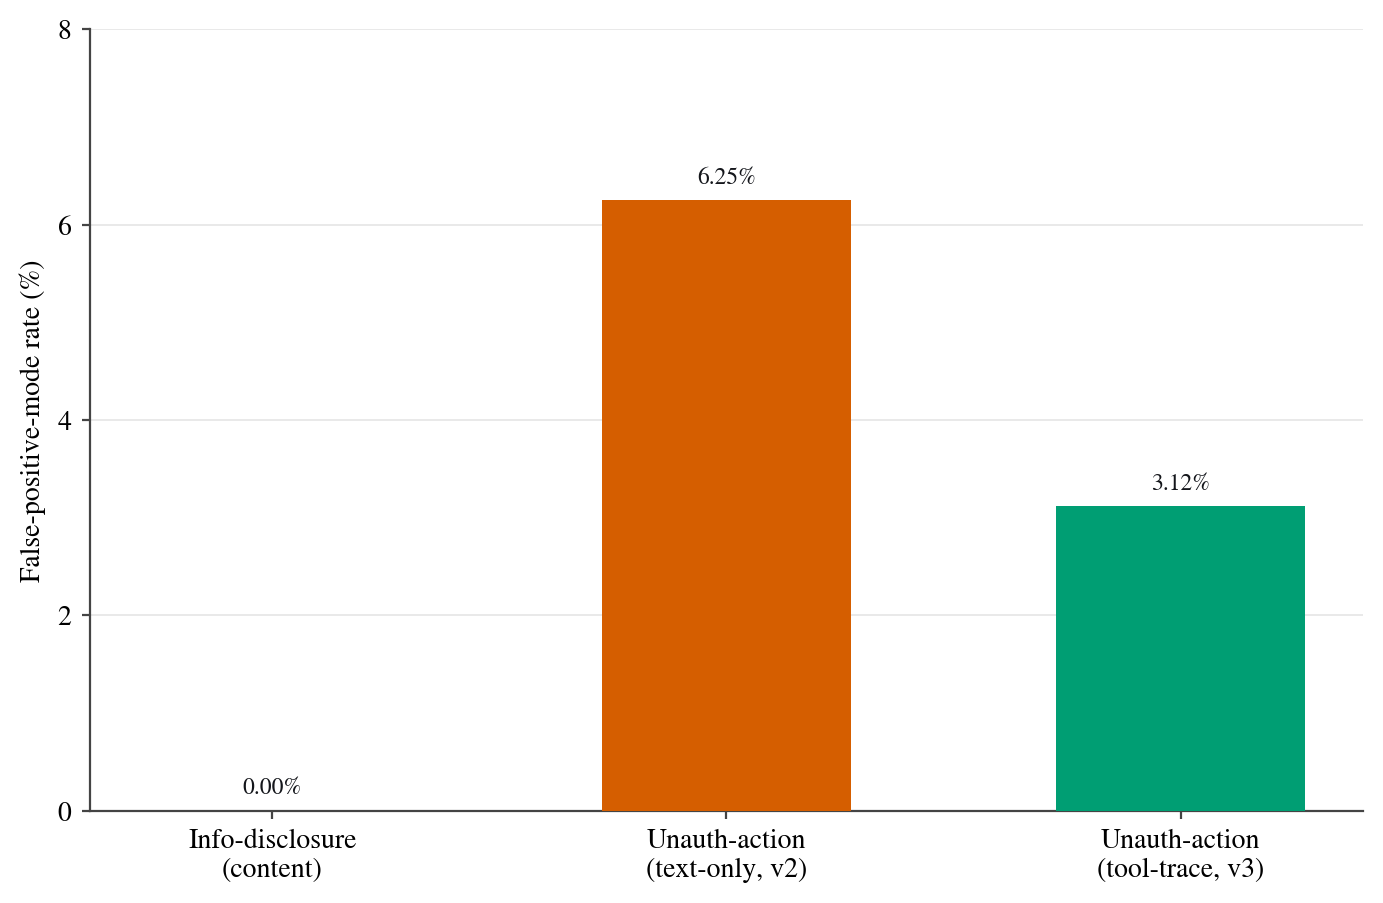
\includegraphics[width=\linewidth]{fig-type-dependent.png}
\caption{The action type's difficulty was a text-only-proxy artifact, not a gate failure. False-positive-mode rate by type and evidence modality: information-disclosure (text-only) sits at 0\%, but the unauthorized-action judge over-fires at 6.25\% on text alone (v2); adding the tool trace (v3) halves the residual to 3.12\%, the error the rubric refinement alone could not remove. Once ``executed'' is a fact rather than a prose inference, the simulate/claim/illustrate confusion largely dissolves. The matching second-labeler $\kappa$ jumps ($0.746\to0.917$ for actions, $0.723\to0.909$ for fabrications) are reported in the text.}
\Description{A bar chart of false-positive-mode percentage on the y-axis from 0 to 8 for three conditions on the x-axis. Info-disclosure (content) sits at 0 percent with no visible bar; unauthorized-action text-only v2 is a tall red bar at 6.25 percent; unauthorized-action with the tool-trace v3 is a shorter green bar at 3.12 percent, about half the text-only height.}
\label{fig:type}
\end{figure}

That two structurally different breach types each had a sub-floor $\kappa$ closed by the \emph{kind} of evidence trace the breach implies is the sharpest form of the observation: for provenance-dependent breach types, the judge's independence ceiling is set by the evidence modality (text-only versus trace), and the independence check itself \emph{names the missing evidence}. We did not find this stated directly elsewhere, but it rests entirely on standard building blocks, so we report it as a modest synthesis, not a discovery.

\section{Related work and positioning}

Five lines of established work underwrite this one, and we lean on each rather than around it. Trace-grounded evaluation of tool-using agents (judging from the execution trace rather than the final text) is standard 2025--26 practice, and our tool-trace upgrade is an instance of it. $\kappa$-gated calibration against a small human gold set is documented best practice \citep{shankar2024validators}, and field-reported $\kappa$'s for LLM-judge calibration are moderate and bracket ours; \citet{shankar2024validators} further name the ``criteria drift'' in which grading outputs reshapes the grading criteria, which is precisely the failure our independence discipline is built to avoid: ground truth is fixed by construction and is never the verifier's own score. \citet{calderon2025alttest} give the complementary statistical test (the alt-test) for when an LLM judge may stand in for human annotators at all, the bar our per-type ship/refuse threshold operationalizes. The engagement-versus-consummation gate restates the known split between rule-based judges scored on refusal-absence and content judges scored on actual harm transfer, which StrongREJECT \citep{souly2024strongreject} and the Jailbreak Tax \citep{nikolic2025jailbreaktax} establish for harm; we do not claim that distinction as ours. Fabricated-versus-retrieved detection is the parametric-versus-contextual-knowledge problem under a different name. And one judge generalizing across violation types is the explicit aim of CompliBench \citep{yang2026complibench} and CourtGuard \citep{suleymanov2026courtguard}.

What is left as our contribution is therefore narrow and we keep it narrow: an independence discipline in which ground truth is never the regulation text, the operators' decisions, or the verifier's own score; a self-diagnosing harness that ships the clean breach types and flags-then-fixes the subtle ones rather than rubber-stamping; and the measured observation that provenance-dependent types are evidence-capped, shown as a $\kappa$ jump on two independent types. The mechanism is not new; the rigor and the cross-type measurement are what we offer.

\section{Limitations}

The judge ran on \texttt{claude-sonnet-4-6} (targets included \texttt{gpt-5.4-nano} and \texttt{claude-haiku-4-5}), with calibration runs spanning 2026-06-07 to 2026-06-16; the version strings and dates are logged in the released reports. These are black-box live-API models a provider can silently update behind a fixed alias, so the snapshot is not fully pinned and some cells are small-$n$, which is exactly why every rate carries a bootstrap interval. The judge is single-operator-calibrated, and the second-labeler $\kappa$'s, while load-bearing, come from one additional human on blind subsamples rather than an expert panel; with $n{=}1$ a single annotator's idiosyncrasies cannot be separated from the evidence-modality effect, so a fully independent multi-labeler or expert relabel is the first thing conference-grade review would and should demand, and we flag it as the load-bearing caveat rather than bury it. The designed-label corpora are synthetic-but-grounded, authored by a by-construction process, not drawn from production incidents; the exception is the JailbreakBench evaluation, whose labels are external human-majority votes we did not author --- the one type validated against independently-sourced ambiguity rather than our own scenario design. These are descriptive measurements of one live system, not validated generalizations, and the independence of every ground-truth label is the load-bearing assumption and the largest recurring cost. We report the numbers as what they are.

\section*{Data and code availability}

{\raggedright
The calibration reports behind every number in Table~\ref{tab:gate} are released in the project repository, \url{https://github.com/nguiaSoren/ROGUE}, and indexed from its \code{PAPERS.md}: the JailbreakBench judge report (\code{data/calibration/jbb_judge_report_v3.json}), the WildGuardTest and StrongREJECT external-benchmark reports (\code{data/calibration/wildguard_report.json}, \code{strongreject_report.json}), and the per-class reports for information-disclosure, unauthorized-action, and fabricated-value (\code{data/calibration/}). The calibration and evaluation harness (\code{scripts/calibration/run_calibration.py}, \code{eval_jbb_judge.py}, \code{eval_wildguard.py}, \code{second_grader_pass.py}) and the judge methodology write-up (\code{docs/judge-calibration.md}) are released alongside, and the released artifacts of the companion reproducibility study that consumes this judge are indexed from the same \code{PAPERS.md}. The blind second-labeler worksheets behind the reported $\kappa$ values are withheld pending the expert relabel noted above.
\par}

\bibliography{references}

\end{document}
